\documentclass{article}

\usepackage[utf8]{inputenc}
\usepackage[spanish,es-lcroman]{babel}
\usepackage{fancyhdr}
\usepackage{lastpage}
\usepackage{extramarks}
\usepackage[usenames,dvipsnames]{color}
\usepackage{graphicx}
\usepackage{listings}
\usepackage{xparse}
\usepackage{courier}
\usepackage{amsmath}
\usepackage{enumitem}
\usepackage{hyperref}
\hypersetup{
    colorlinks=true,
    linkcolor=blue,
    urlcolor=blue,
    linktoc=all
}

\setenumerate[1]{label=(\alph*)}

% Margenes
\topmargin=-0.65in
\evensidemargin=0in
\oddsidemargin=0in
\textwidth=6.5in
\textheight=9.0in
\headsep=0.25in

% Header y footer
\pagestyle{fancy}
\lhead{}
\chead{\tareaRamo\ (\tareaProfesor): \tareaTitulo} % Centro
\rhead{\firstxmark}
\lfoot{\lastxmark}
\cfoot{}
\rfoot{Página\ \thepage\ de\ \protect\pageref{LastPage}} % Pagina
\renewcommand\headrulewidth{0.4pt}
\renewcommand\footrulewidth{0.4pt}

\setlength\parindent{0pt} % Eliminar la indentación

\newcommand{\python}[2]{
\begin{itemize}
\item[]\lstinputlisting[language=Python,caption=#2,label=#1]{#1.py}
\end{itemize}
}

%----------------------------------------------------------------------------------------
%	Meta Información
%----------------------------------------------------------------------------------------
\newcommand{\tareaTitulo}{Tarea\ \#3 - Informe} % titulo del informe
\newcommand{\tareaFecha}{\today} % Fecha
\newcommand{\tareaRamo}{Redes de Computadores} % Ramo
\newcommand{\tareaUniversidad}{Departamento\ de\ Informática\ UTFSM, Santiago} %usm
\newcommand{\tareaProfesor}{Oscar\ Encina} % Profesor
\newcommand{\tareaAyudante}{Alex\ Arenas} % Ayudante
\newcommand{\tareaAlumnoUno}{Eduardo\ Fernandez\ S.} % Nombre Alumno 1
\newcommand{\tareaAlumnoDos}{Victor Cifuentes S.} % Nombre Alumno 2
\newcommand{\tareaRolUno}{201004301-0} % Rol alumno 1
\newcommand{\tareaRolDos}{201073557-5} % Rol Alumno 2

%----------------------------------------------------------------------------------------
%	Título
%----------------------------------------------------------------------------------------

\title{
\textmd{\textbf{\tareaRamo:\ \tareaTitulo}}\\
\normalsize\vspace{0.1in}\small{\tareaFecha}\\
\vspace{0.1in}\large{Profesor: \textit{\tareaProfesor} \qquad \qquad Ayudante: \textit{\tareaAyudante}}
}

\author{
    \textbf{\tareaAlumnoUno} \\
    \small{\tareaRolUno}
    \and
    \textbf{\tareaAlumnoDos} \\
    \small{\tareaRolDos}}
\date{}

%----------------------------------------------------------------------------------------

\begin{document}

\maketitle

\section{Pregunta 1: Open Visual TraceRouter}	

En esta secci\'on se analizar\'an 5 direcciones donde se describir\'a el viaje de los paquetes y las rutas que toman.\\

Los paquetes viajan a trav\'es de routers (saltos) para poder conectarse a internet. En el caso de Chile las conexiones se realizar\'an a trav\'es de 2 NAP en Miami, las cuales est\'an conectadas con nosotros a trav\'es de fibra \'optica que van por el oc\'eano y llegan de los ISP las distribuidoras y de ah\'i a conexiones residenciales para finalmente llegar al dispositivo. Por otra parte el request llega al DNS center a trav\'es de la IP, el DNS lo redirecciona al servidor correspondiente y eso manda finalmente los paquetes. Cabe decir que los proveedores de servicios est\'an conectados a trav\'es de los diferentes Tier que est\'an en la capa mas alta de la jerarqu\'ia de Internet.\\

Usando $Open Visual Tracerouter$ se obtienen las siguientes im\'agenes para cada direcci\'on:

\begin{itemize}
\item http://moodle.inf.utfsm.cl\\

\begin{center}$
\begin{array}{c}
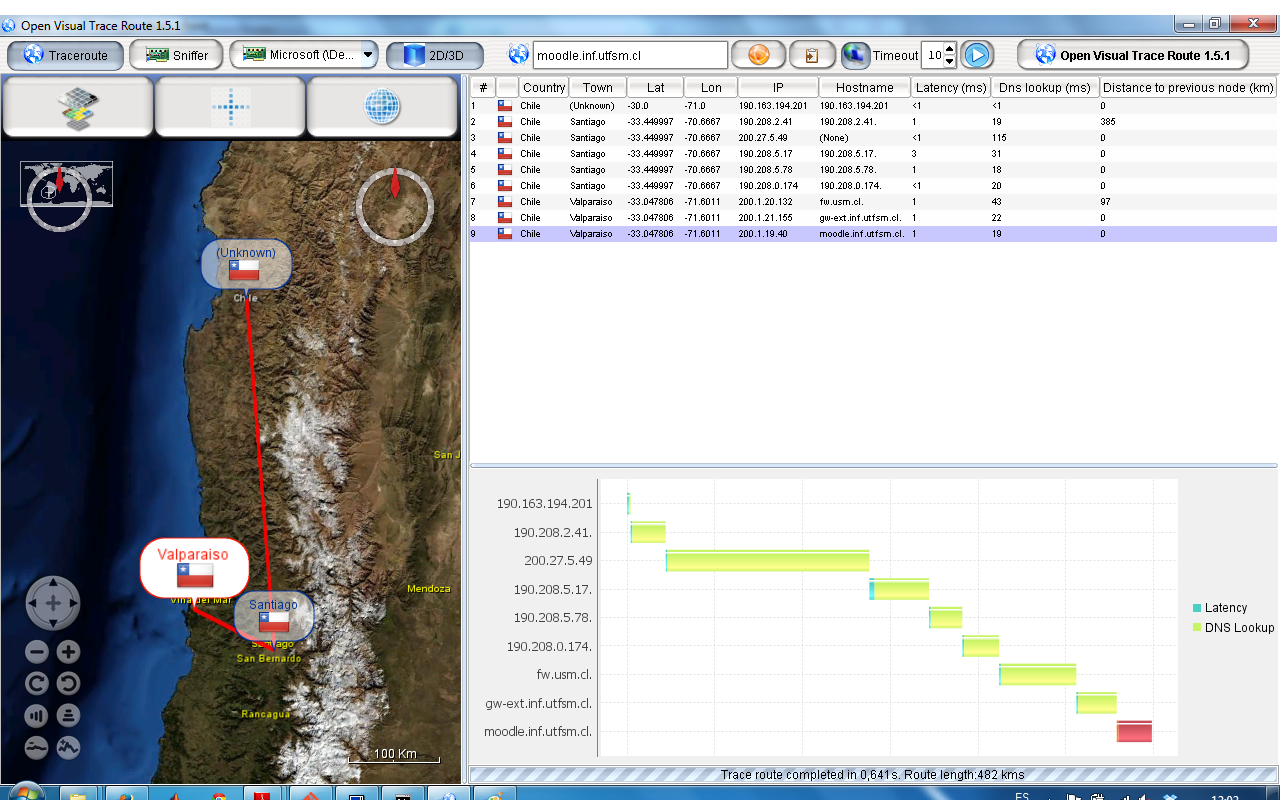
\includegraphics[width=6in]{Redes_moodle_TR.png}
\end{array}$
\end{center}
En esta direcci\'on los paquetes viajan a trav\'es de 9 routers (incluyendo el local, es decir, desde donde se intenta conectar a internet), todos provenientes de Chile. 

\item http://google.cl\\

\begin{center}$
\begin{array}{c}
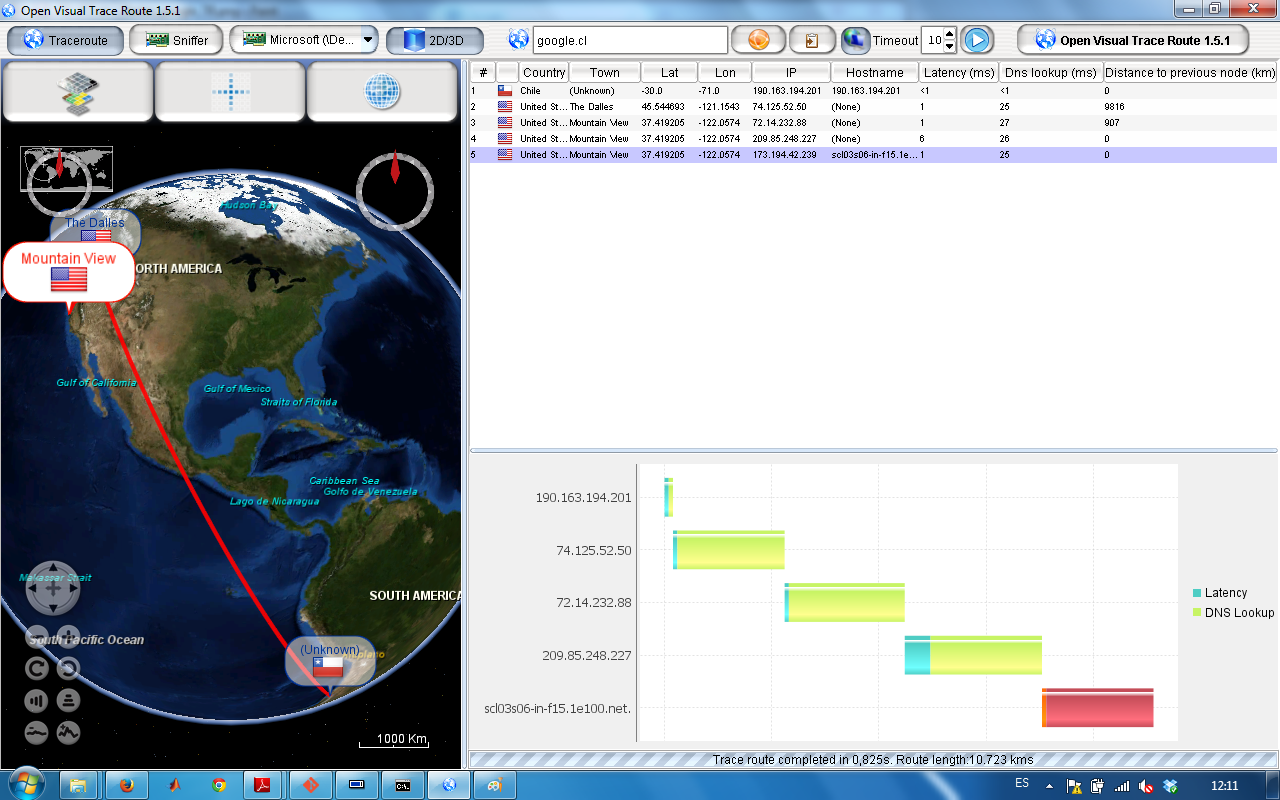
\includegraphics[width=6in]{Redes_google_TR.png}
\end{array}$
\end{center}
En esta direcci\'on los paquetes viajan por un router proveniente de Chile (local) y, adem\'as, por 4 routers provenientes de Estados Unidos.

\item http://cime.cl\\

\begin{center}$
\begin{array}{c}
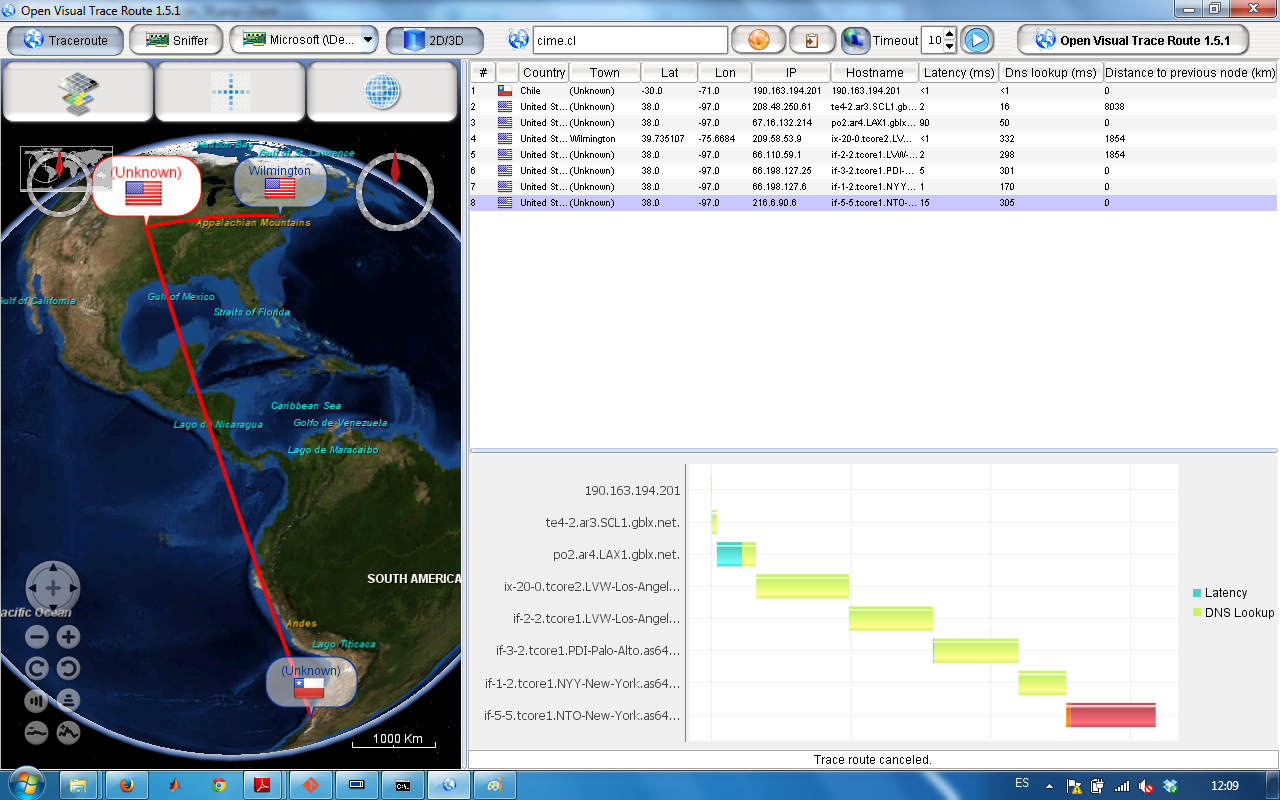
\includegraphics[width=6in]{Redes_cime_TR.png}
\end{array}$
\end{center}
En esta direcci\'on los paquetes viajan por un router proveniente de Chile (local) y, adem\'as, por 7 routers provenientes de Estados Unidos.

\item http://wikipedia.com\\

\begin{center}$
\begin{array}{c}
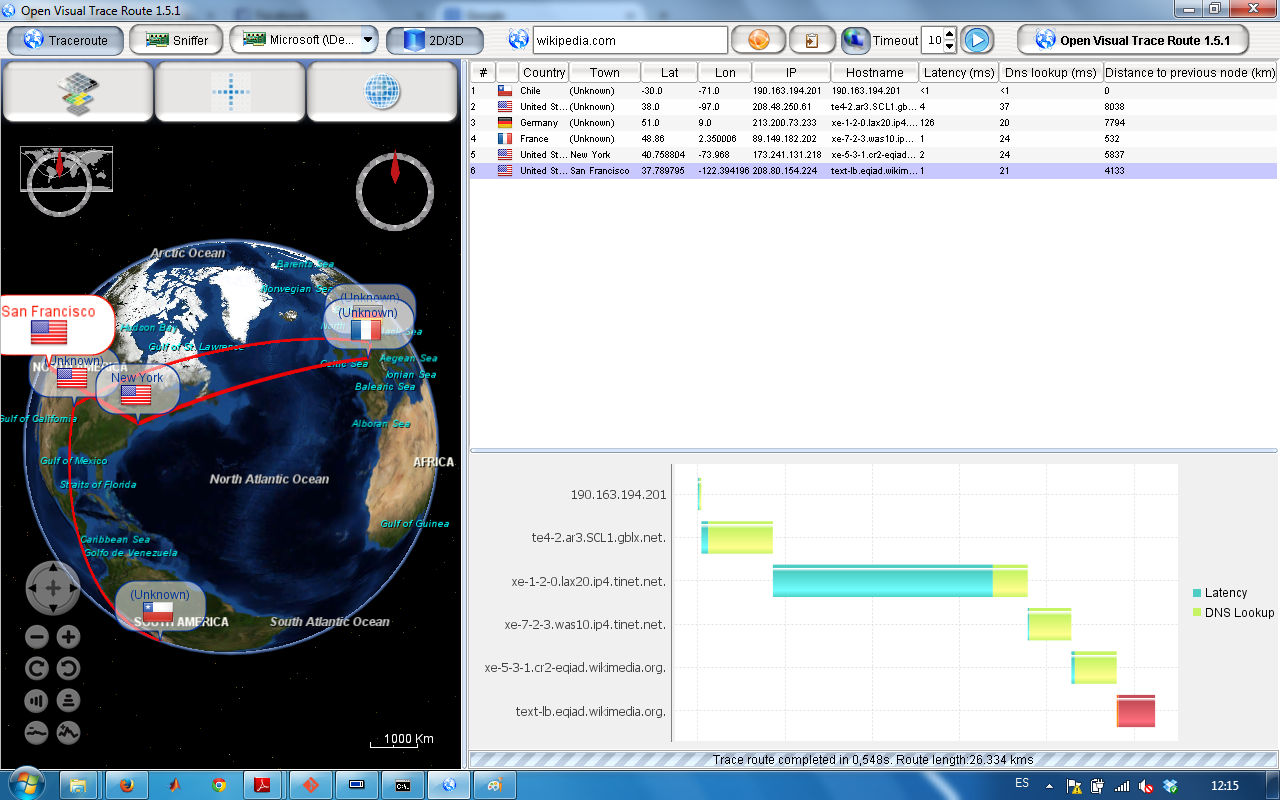
\includegraphics[width=6in]{Redes_wikipedia_TR.png}
\end{array}$
\end{center}
En esta direcci\'on los paquetes viajan por distintos paises por 6 routers distintos: Chile (local), Alemania, Francia y Estados Unidos (3 routers).

\item http://www.chile.embassy.gov.au\\

\begin{center}$
\begin{array}{c}
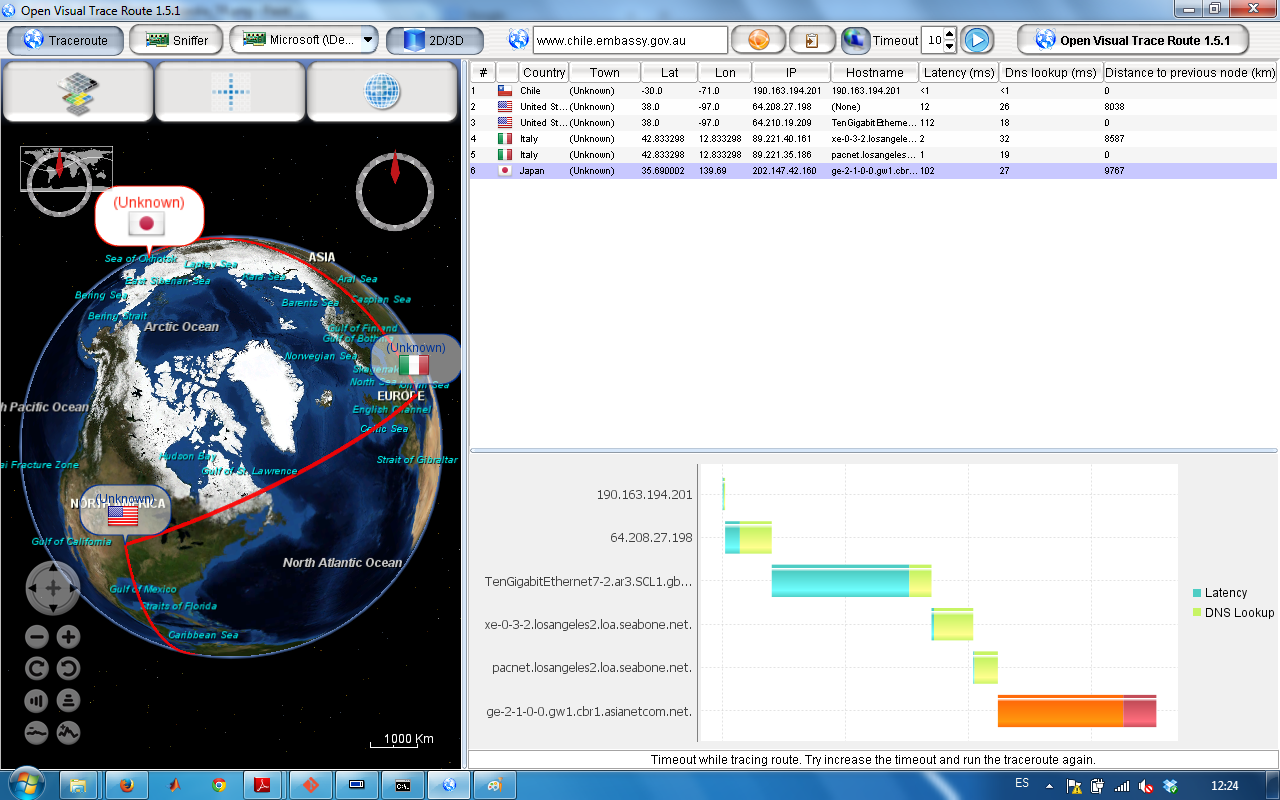
\includegraphics[width=6in]{Redes_chile-embassy_TR.png}
\end{array}$
\end{center}
En esta direcci\'on los paquetes viajan por distintos paises para poder conectarse a internet, pasando por 6 routers: Chile (local), Estados Unidos (2 routers), Italia (2 routers) y Jap\'on.\\

Cada una de las direcciones toman las rutas mostradas (y pueden ser diferentes) con el objetivo de transferir paquetes a un menor costo, es decir, menor distancia, tiempo, etc. En otras palabras, se trata de obtener una transferencia de paquetes de manera eficiente.\\

Como dato extra, una diferencia entre Moodle y los dem\'as es que implement\'o un sistema llamado MUC, o Universal Cache Moodle que permite que ciertas funciones de Moodle (por ejemplo, cadena de obtenci\'on) se aprovechan de los servicios instalados por cada persona o instituci\'on a la que Moodle le presta servicios y guarda informaci\'on de Moodle (por ejemplo, archivos de cach\'e, memoria RAM, memcached), es por esto que para el caso de moodle, Traceroute no traza una ruta m\'as lejana, ya que, es este servicio el que funciona distinto a los dem\'as.

\end{itemize}

\section{Pregunta 2: Algoritmo Vector-distancia}

\begin{figure}[ht!]
\centering
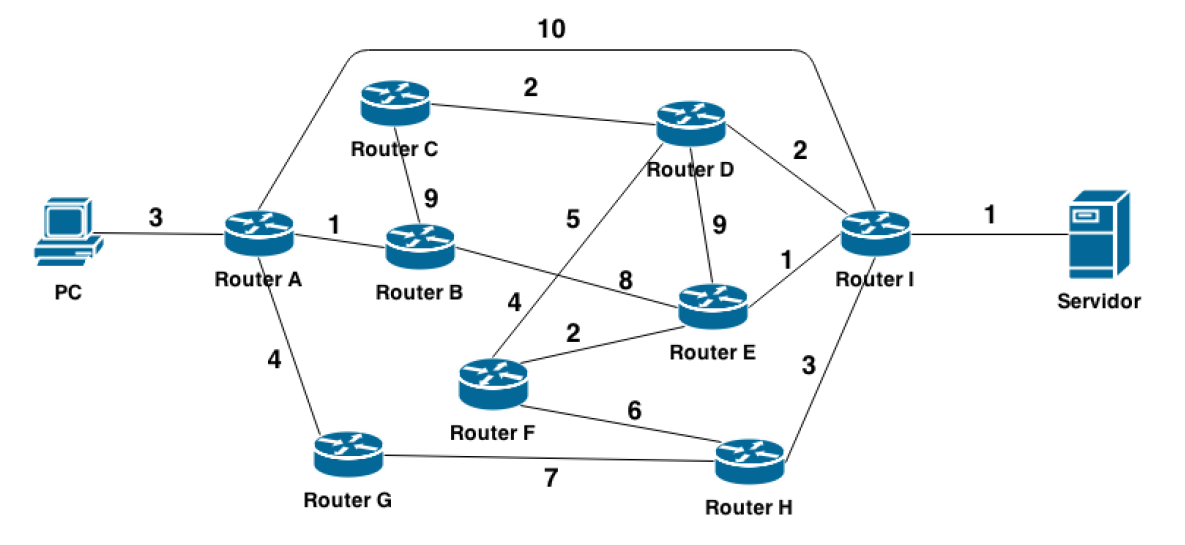
\includegraphics[width=130mm]{red1.PNG}
\caption{Red a menor escala.}
\label{overflow}
\end{figure}

Para el c\'alculo de los menores costos de todos los routers, se realiza el algoritmo de Vector-distancia para encontrar las tablas de todos los costos de todos los routers. El procedimiento es el siguiente: desde un router, se calcula el vector distancia estimada desde \'este a sus routers vecinos, luego esos vecinos avisa a sus vecinos respectivos actualizando su distancia por medio de la siguiente f\'ormula (ecuaci\'on de Bellman-Ford):\\

$D_x$($y$)=min\{$c(x,v)$+$D_v$(y),...\}
\\

Este algoritmo continua hasta que todos los routers convergan a un valor, el cual corresponde al menor costo de ir de un router a los dem\'as.\\

Tabla inicial:\\
\begin{tabular}{||l | c | c | c | c | c | c | c | c | c | c | c ||}
\hline
\hline
O/D & PC & A & B & C & D & E & F & G & H & I & SERVER \\
\hline
PC & 0 & 3 & $\infty$ & $\infty$ & $\infty$ & $\infty$ & $\infty$ & $\infty$ & $\infty$ & $\infty$ & $\infty$ \\
\hline
A & 3 & 0 & 1 & $\infty$ & $\infty$ & $\infty$ & $\infty$ & 4 & $\infty$ & 10 & $\infty$ \\
\hline
B & $\infty$ & 1 & 0 & 9 & $\infty$ & $\infty$ & $\infty$ & $\infty$ & $\infty$ & $\infty$ & $\infty$ \\
\hline
C & $\infty$ & $\infty$ & 9 & 0 & 2 & $\infty$ & $\infty$ & $\infty$ & $\infty$ & $\infty$ & $\infty$ \\
\hline
D & $\infty$ & $\infty$ & $\infty$ & 2 & 0 & 9 & 4 & $\infty$ & $\infty$ & 2 & $\infty$ \\
\hline
E & $\infty$ & $\infty$ & 8 & $\infty$ & 9 & 0 & 2 & $\infty$ & $\infty$ & $\infty$ & $\infty$ \\
\hline
F & $\infty$ & $\infty$ & $\infty$ & $\infty$ & 4 & 2 & 0 & $\infty$ & 6 & $\infty$ & $\infty$ \\
\hline
G & $\infty$ & 4 & $\infty$ & $\infty$ & $\infty$ & $\infty$ & $\infty$ & 0 & 7 & $\infty$ & $\infty$ \\
\hline
H & $\infty$ & $\infty$ & $\infty$ & $\infty$ & $\infty$ & $\infty$ & 6 & 7 & 0 & 3 & $\infty$ \\
\hline
I & $\infty$ & 10 & $\infty$ & $\infty$ & 2 & 1 & $\infty$ & $\infty$ & 3 & 0 & 1 \\
\hline
SERVER & $\infty$ & $\infty$ & $\infty$ & $\infty$ & $\infty$ & $\infty$ & $\infty$ & $\infty$ & $\infty$ & 1 & 0 \\
\hline
\end{tabular}\\

Tabla de costos despu\'es de la primera iteraci\'on:\\
\begin{tabular}{||l | c | c | c | c | c | c | c | c | c | c | c ||}
\hline
\hline
O/D & PC & A & B & C & D & E & F & G & H & I & SERVER \\
\hline
PC & 0 & 3 & 4 & $\infty$ & $\infty$ & $\infty$ & $\infty$ & 7 & $\infty$ & 13 & $\infty$ \\
\hline
A & 3 & 0 & 1 & 10 & 12 & 9 & $\infty$ & 4 & 11 & 10 & 11 \\
\hline
B & 4 & 1 & 0 & 9 & 11 & 8 & 10 & 5 & $\infty$ & 9 & $\infty$ \\
\hline
C & $\infty$ & 10 & 9 & 0 & 2 & 11 & 6 & $\infty$ & $\infty$ & 4 & $\infty$ \\
\hline
D & $\infty$ & $\infty$ & 11 & 2 & 0 & 3 & 4 & $\infty$ & 5 & 2 & 3 \\
\hline
E & $\infty$ & 9 & 8 & 11 & 3 & 0 & 2 & $\infty$ & 4 & 1 & 2 \\
\hline
F & $\infty$ & $\infty$ & 10 & 6 & 4 & 2 & 0 & 13 & 6 & 3 & $\infty$ \\
\hline
G & 7 & 4 & 5 & $\infty$ & $\infty$ & $\infty$ & 13 & 0 & 7 & 10 & $\infty$ \\
\hline
H & $\infty$ & 11 & $\infty$ & $\infty$ & 5 & 4 & 6 & 7 & 0 & 3 & 4 \\
\hline
I & 13 & 10 & 9 & 4 & 2 & 1 & 3 & 10 & 3 & 0 & 1 \\
\hline
SERVER & $\infty$ & 11 & $\infty$ & $\infty$ & 3 & 2 & $\infty$ & $\infty$ & 4 & 1 & 0 \\
\hline
\end{tabular}\\\\

$D_i$(PC)=min\{c(I,A)+D1(PC),c(I,D)+Dd(PC),c(I,E)+De(PC),c(I,H)+Dh(PC),C(I,S+Ds(PC))\}=13\\
$D_i$(A)=min\{10,$\infty$,$\infty$\}=10\\
$D_i$(B)=min\{11,$\infty$,9,$\infty$,$\infty$\}=9\\
$D_i$(C)=min\{$\infty$,4,$\infty$,$\infty$,$\infty$\}=4\\
$D_i$(D)=min\{$\infty$,2,10,$\infty$,$\infty$\}=2\\
$D_i$(E)=min\{$\infty$,11,1,$\infty$,$\infty$\}=1\\
$D_i$(F)=min\{$\infty$,6,3,9,$\infty$\}=3\\
$D_i$(G)=min\{14,$\infty$,$\infty$,10,$\infty$\}=10\\
$D_i$(H)=min\{$\infty$,$\infty$,$\infty$,3,$\infty$\}=3\\
$D_i$(SERVER)=1\\


$D_a$(PC)=min\{c(A,PC)+Dpc(PC),c(A,B)+Db(PC),c(A,G)+Dg(PC),c(A,I)+Di(PC)\}=3\\
$D_a$(B)=min\{$\infty$,1,$\infty$,$\infty$\}=1
$D_a$(C)=min\{$\infty$,10,$\infty$,$\infty$\}=10\\
$D_a$(D)=min\{$\infty$,$\infty$,$\infty$,12\}=12\\
$D_a$(E)=min\{$\infty$,9,$\infty$,11\}=9\\
$D_a$(F)=min\{$\infty$,$\infty$,$\infty$,$\infty$\}=$\infty$\\
$D_a$(G)=min\{$\infty$,$\infty$,4,$\infty$\}=4\\
$D_a$(H)=min\{$\infty$,$\infty$,11,13\}=11\\
$D_a$(I)=min\{$\infty$,$\infty$,$\infty$,10\}=10\\
$D_a$(SERVER)=11\\


$D_d$(PC)=min\{c(D,C)+Dc(PC),c(D,E)+Df(PC),c(D,I)+Di(PC)\}=$\infty$\\
$D_d$(B)=min\{$\infty$,$\infty$,$\infty$,$\infty$\}=$\infty$\\
$D_d$(C)=min\{11,17,$\infty$,$\infty$\}=11\\
$D_d$(D)=min\{2,$\infty$,$\infty$,$\infty$\}=2\\
$D_d$(E)=min\{$\infty$,9,6,3\}=3\\
$D_d$(F)=min\{$\infty$,11,4,$\infty$\}=4\\
$D_d$(G)=min\{$\infty$,$\infty$,$\infty$,$\infty$\}=$\infty$\\
$D_d$(H)=min\{$\infty$,$\infty$,10,5\}=5\\
$D_d$(I)=min\{$\infty$,10,$\infty$,2\}=2\\
$D_d$(SERVER)=\{$\infty$,$\infty$,$\infty$,3\}=3\\

$D_e$(PC)=min\{c(E,B)+Db(PC),c(E,D)+db(PC),c(E,F)+Df(PC),c(E,I)+D(PC)\}=$\infty$\\
$D_e$(B)=min\{9,$\infty$,$\infty$,11\}=9\\
$D_e$(C)=min\{8,$\infty$,$\infty$,$\infty$\}=8\\
$D_e$(D)=min\{17,11,$\infty$,$\infty$\}=11\\
$D_e$(E)=min\{$\infty$,9,6,3\}=3\\
$D_e$(F)=min\{$\infty$,13,2,$\infty$\}=2\\
$D_e$(G)=min\{$\infty$,$\infty$,$\infty$,$\infty$\}=$\infty$\\
$D_e$(H)=min\{$\infty$,$\infty$,$\infty$,4\}=4\\
$D_e$(I)=min\{$\infty$,11,$\infty$,1\}=1\\
$D_e$(SERVER)=\{$\infty$,$\infty$,$\infty$,2\}=2\\

$D_b$(PC)=min\{c(B,A)+Da(PC),c(B,C)+Dc(PC),c(B,E)+De(PC)\}=4\\
$D_b$(A)=min\{1,$\infty$,$\infty$\}=1\\
$D_b$(C)=min\{$\infty$,9,$\infty$\}=9\\
$D_b$(D)=min\{$\infty$,11,17\}=11\\
$D_b$(E)=min\{$\infty$,$\infty$,8\}=8\\
$D_b$(F)=min\{$\infty$,$\infty$,10\}=10\\
$D_b$(G)=min\{5,$\infty$,$\infty$\}=5\\
$D_b$(H)=min\{$\infty$,$\infty$,$\infty$\}=$\infty$\\
$D_b$(I)=min\{$\infty$,$\infty$,9\}=9\\
$D_b$(SERVER)=min\{$\infty$,$\infty$,$\infty$\}=$\infty$\\

$D_f$(PC)=min\{c(F,D)+Db(PC),c(F,E)+De(PC),c(H,I)+Di(PC)\}=$\infty$\\
$D_f$(A)=min\{$\infty$,$\infty$,$\infty$\}=$\infty$\\
$D_f$(B)=min\{$\infty$,10,$\infty$\}=10\\
$D_f$(C)=min\{6,$\infty$,$\infty$\}=6\\
$D_f$(D)=min\{4,11,$\infty$\}=4\\
$D_f$(E)=min\{13,2,$\infty$\}=2\\
$D_f$(G)=min\{$\infty$,$\infty$\,13\}=13\\
$D_f$(H)=min\{$\infty$,$\infty$,6\}=6\\
$D_f$(I)=min\{$\infty$,3,9\}=3\\
$D_f$(SERVER)=min\{$\infty$,$\infty$,$\infty$\}=$\infty$\\

$D_h$(PC)=min\{c(H,F)+Df(PC),c(H,G)+De(PC),c(H,I)+Di(PC)\}=$\infty$\\
$D_h$(A)=min\{$\infty$,11,$\infty$\}=11\\
$D_h$(B)=min\{$\infty$,10,$\infty$\}=$\infty$\\
$D_h$(C)=min\{$\infty$,$\infty$,$\infty$\}=$\infty$\\
$D_h$(D)=min\{10,$\infty$,5\}=5\\
$D_h$(E)=min\{8,$\infty$,4\}=4\\
$D_h$(F)=min\{6,$\infty$,$\infty$\}=6\\
$D_h$(G)=min\{$\infty$,7,$\infty$\}=7\\
$D_h$(I)=min\{$\infty$,$\infty$,3\}=3\\
$D_h$(SERVER)=min\{$\infty$,$\infty$,4\}=4\\\\\\

$D_c$(PC)=min\{c(H,F)+Df(PC),c(H,G)+De(PC),c(H,I)+Di(PC)\}=$\infty$\\
$D_c$(A)=min\{$\infty$,11,$\infty$\}=11\\
$D_c$(B)=min\{$\infty$,10,$\infty$\}=$\infty$\\
$D_c$(C)=min\{$\infty$,$\infty$,$\infty$\}=$\infty$\\
$D_c$(D)=min\{10,$\infty$,5\}=5\\
$D_c$(E)=min\{8,$\infty$,4\}=4\\
$D_c$(F)=min\{6,$\infty$,$\infty$\}=6\\
$D_c$(G)=min\{$\infty$,7,$\infty$\}=7\\
$D_c$(I)=min\{$\infty$,$\infty$,3\}=3\\
$D_c$(SERVER)=min\{$\infty$,$\infty$,4\}=4\\

$D_g$(PC)=min\{c(G,A)+Da(PC),c(G,H)+Dh(PC)\}=7\\
$D_g$(A)=min\{4,$\infty$\}=4\\
$D_g$(B)=min\{5,$\infty$\}=5\\
$D_g$(C)=min\{$\infty$,$\infty$\}=$\infty$\\
$D_g$(D)=min\{$\infty$,$\infty$\}=$\infty$\\
$D_g$(E)=min\{$\infty$,$\infty$\}=$\infty$\\
$D_g$(F)=min\{$\infty$,13\}=13\\
$D_g$(H)=min\{$\infty$,7\}=7\\
$D_g$(I)=min\{14,10\}=10\\
$D_g$(SERVER)=min\{$\infty$,$\infty$\}=$\infty$\\

$D_{pc}$(A)=min\{c(PC,A)+Da(PC)\}=3\\
$D_{pc}$(B)=4\\
$D_{pc}$(C)=$\infty$\\
$D_{pc}$(D)=$\infty$\\
$D_{pc}$(E)=$\infty$\\
$D_{pc}$(F)=$\infty$\\
$D_{pc}$(G)=7\\
$D_{pc}$(H)=$\infty$\\
$D_{pc}$(I)=13\\
$D_{pc}$(SERVER)=$\infty$\\

$D_s$(PC)=min\{c(S,I)+Di(PC)\}=$\infty$\\
$D_s$(A)=11\\
$D_s$(B)=$\infty$\\
$D_s$(C)=$\infty$\\
$D_s$(D)=3\\
$D_s$(E)=2\\
$D_s$(F)=$\infty$\\
$D_s$(G)=$\infty$\\
$D_s$(H)=4\\
$D_s$(I)=1\\\\\\

Tabla de costos despu\'es de la segunda iteraci\'on:\\
\begin{tabular}{||l | c | c | c | c | c | c | c | c | c | c | c ||}
\hline
\hline
O/D & PC & A & B & C & D & E & F & G & H & I & SERVER \\
\hline
PC & 0 & 3 & 4 & 13 & 15 & 12 & $\infty$ & 7 & 14 & 13 & 14 \\
\hline
A & 3 & 0 & 1 & 10 & 12 & 9 & 11 & 4 & 11 & 10 & 11 \\
\hline
B & 4 & 1 & 0 & 9 & 11 & 8 & 10 & 5 & 12 & 9 & 10 \\
\hline
C & 13 & 10 & 9 & 0 & 2 & 5 & 6 & 14 & 7 & 4 & 5 \\
\hline
D & 15 & 12 & 11 & 2 & 0 & 3 & 4 & 12 & 5 & 2 & 3 \\
\hline
E & 12 & 9 & 8 & 5 & 3 & 0 & 2 & 11 & 4 & 1 & 2 \\
\hline
F & $\infty$ & 11 & 10 & 6 & 4 & 2 & 0 & 13 & 6 & 3 & 4 \\
\hline
G & 7 & 4 & 5 & 14 & 12 & 11 & 13 & 0 & 7 & 10 & 11 \\
\hline
H & 14 & 11 & 12 & 7 & 5 & 4 & 6 & 7 & 0 & 3 & 4 \\
\hline
I & 13 & 10 & 9 & 4 & 2 & 1 & 3 & 10 & 3 & 0 & 1 \\
\hline
SERVER & 14 & 11 & 10 & 5 & 3 & 2 & 4 & 11 & 4 & 1 & 0 \\
\hline
\end{tabular}\\\\

$D_{pc}$(A)=3\\
$D_{pc}$(B)=4\\
$D_{pc}$(C)=13\\
$D_{pc}$(D)=15\\
$D_{pc}$(E)=12\\
$D_{pc}$(F)=$\infty$\\
$D_{pc}$(G)=7\\
$D_{pc}$(H)=14\\
$D_{pc}$(I)=13\\
$D_{pc}$(SERVER)=14\\

$D_a$(PC)=3\\
$D_a$(B)=1\\
$D_a$(C)=min{$\infty$,10,$\infty$,14\}=10\\
$D_a$(D)=min\{$\infty$,12,$\infty$,12\}=12\\
$D_a$(E)=min\{$\infty$,9,$\infty$,11\}=9\\
$D_a$(F)=min\{$\infty$,11,17,13\}=11\\
$D_a$(G)=4\\
$D_a$(H)=min\{$\infty$,$\infty$,11,13\}=11\\
$D_a$(I)=min\{$\infty$,10,14,10\}=10\\
$D_a$(SERVER)=min\{$\infty$,$\infty$,$\infty$,11\}=11\\

$D_b$(PC)=4\\
$D_b$(A)=1\\
$D_b$(C)=min{$\infty$,9,19\}=9\\
$D_b$(D)=min\{13,20,11\}=11\\
$D_b$(E)=min\{10,20,,8\}=8\\
$D_b$(F)=min\{$\infty$,15,10\}=10\\
$D_b$(G)=min\{5,$\infty$,$\infty$\}=5\\
$D_b$(H)=min\{12,$\infty$,12\}=12\\
$D_b$(I)=min\{11,13,9\}=9\\
$D_b$(SERVER)=min\{12,$\infty$,10\}=10\\

$D_c$(PC)=min{13,$\infty$\}=13\\
$D_c$(A)=10\\
$D_c$(C)=min\{9,13\}=9\\
$D_c$(D)=2\\
$D_c$(E)=min\{17,5\}=5\\
$D_c$(F)=min\{19,6\}=6\\
$D_c$(G)=min\{14,$\infty$\}=14\\
$D_c$(H)=min\{$\infty$,7\}=7\\
$D_c$(I)=min\{18,4\}=4\\
$D_c$(SERVER)=min\{$\infty$,5\}=5\\

$D_d$(PC)=min\{$\infty$,$\infty$,$\infty$,15\}=15\\
$D_d$(A)=min\{12,18,$\infty$,12\}=12\\
$D_d$(B)=min\{11,17,14,11\}=11\\
$D_d$(C)=min\{2,...\}=15\\
$D_d$(E)=min\{13,3\}=3\\
$D_d$(F)=min\{8,11,4,5\}=4\\
$D_d$(G)=min\{$\infty$,$\infty$,17,12\}=12\\
$D_d$(H)=min\{$\infty$,13,10,5\}=5\\
$D_d$(I)=min\{...,2\}=2\\
$D_d$(SERVER)=min\{...,3\}=3\\

$D_e$(PC)=min\{12,$\infty$,$\infty$,15\}=12\\
$D_e$(A)=min\{9,18,$\infty$,14\}=14\\
$D_e$(B)=min\{8,20,12,10\}=8\\
$D_e$(C)=min\{17,11,8,5\}=5\\
$D_e$(D)=min\{19,9,7,3\}=3\\
$D_e$(F)=min\{18,13,2,4\}=2\\
$D_e$(G)=min\{13,$\infty$,15,11\}=11\\
$D_e$(H)=min\{$\infty$,14,8,4\}=4\\
$D_e$(I)=min\{...\}=1\\
$D_e$(SERVER)=min\{...\}=2\\

$D_f$(PC)=min\{$\infty$,$\infty$,$\infty$\}=$\infty$\\
$D_f$(A)=min\{$\infty$,11,17\}=11\\
$D_f$(B)=min\{15,10,$\infty$\}=10\\
$D_f$(C)=min\{6,13,$\infty$\}=6\\
$D_f$(D)=min\{4,5,11\}=4\\
$D_f$(E)=min\{7,2,10\}=2\\
$D_f$(G)=min\{$\infty$,$\infty$,13\}=13\\
$D_f$(H)=min\{9,6,6\}=6\\
$D_f$(I)=min\{6,3,9\}=3\\
$D_f$(SERVER)=min\{7,4,10\}=4\\

$D_g$(PC)=7\\
$D_g$(A)=4\\
$D_g$(B)=5\\
$D_g$(C)=min\{14,$\infty$\}=14\\
$D_g$(D)=min\{16,12\}=12\\
$D_g$(E)=min\{13,11\}=11\\
$D_g$(F)=min\{$\infty$,13\}=13\\
$D_g$(H)=7\\
$D_g$(I)=min\{14,10\}=10\\
$D_g$(SERVER)=min\{15,11\}=11\\

$D_h$(PC)=min\{$\infty$,14,16\}=14\\
$D_h$(A)=min\{$\infty$,11,13\}=11\\
$D_h$(B)=min\{16,12,12\}=12\\
$D_h$(C)=min\{12,$\infty$,7\}=7\\
$D_h$(D)=min\{10,$\infty$,5\}=5\\
$D_h$(E)=min\{8,$\infty$,4\}=4\\
$D_h$(F)=min\{6,13,6\}=6\\
$D_h$(G)=min\{19,7,13\}=7\\
$D_h$(I)=min\{...\}=3\\
$D_h$(SERVER)=min\{...\}=4\\

$D_i$(PC)=min\{13,$\infty$,$\infty$,$\infty$,$\infty$\}=13\\
$D_i$(A)=min\{10, $\infty$,10,14\}=10\\
$D_i$(B)=min\{11,13,9,$\infty$\}=9\\
$D_i$(C)=4\\
$D_i$(D)=2\\
$D_i$(E)=1\\
$D_i$(F)=3\\
$D_i$(G)=min\{14,$\infty$,$\infty$,10,$\infty$\}=10\\
$D_i$(h)=3\\
$D_i$(SERVER)=1\\

$D_s$(PC)=14\\
$D_s$(A)=11\\
$D_s$(B)=10\\
$D_s$(C)=5\\
$D_s$(D)=3\\
$D_s$(E)=2\\
$D_s$(F)=4\\
$D_s$(G)=11\\
$D_s$(h)=4\\
$D_s$(SERVER)=1\\

Tabla de costos final despu\'es de la tercera iteraci\'on:\\
\begin{tabular}{||l | c | c | c | c | c | c | c | c | c | c | c ||}
\hline
\hline
O/D & PC & A & B & C & D & E & F & G & H & I & SERVER \\
\hline
PC & 0 & 3 & 4 & 13 & 15 & 12 & 14 & 7 & 14 & 13 & 14 \\
\hline
A & 3 & 0 & 1 & 10 & 12 & 9 & 11 & 4 & 11 & 10 & 11 \\
\hline
B & 4 & 1 & 0 & 9 & 11 & 8 & 10 & 5 & 12 & 9 & 10 \\
\hline
C & 13 & 10 & 9 & 0 & 2 & 5 & 6 & 14 & 7 & 4 & 5 \\
\hline
D & 15 & 12 & 11 & 2 & 0 & 3 & 4 & 12 & 5 & 2 & 3 \\
\hline
E & 12 & 9 & 8 & 5 & 3 & 0 & 2 & 11 & 4 & 1 & 2 \\
\hline
F & 14 & 11 & 10 & 6 & 4 & 2 & 0 & 13 & 6 & 3 & 4 \\
\hline
G & 7 & 4 & 5 & 14 & 12 & 11 & 13 & 0 & 7 & 10 & 11 \\
\hline
H & 14 & 11 & 12 & 7 & 5 & 4 & 6 & 7 & 0 & 3 & 4 \\
\hline
I & 13 & 10 & 9 & 4 & 2 & 1 & 3 & 10 & 3 & 0 & 1 \\
\hline
SERVER & 14 & 11 & 10 & 5 & 3 & 2 & 4 & 11 & 4 & 1 & 0 \\
\hline
\end{tabular}\\\\

$D_{pc}$(A)=3\\
$D_{pc}$(B)=4\\
$D_{pc}$(C)=13\\
$D_{pc}$(D)=15\\
$D_{pc}$(E)=12\\
$D_{pc}$(F)=14\\
$D_{pc}$(G)=7\\
$D_{pc}$(H)=14\\
$D_{pc}$(I)=13\\
$D_{pc}$(SERVER)=14\\

\section{Pregunta 3: Rotura de enlace entre los routers H e I}

\begin{figure}[ht!]
\centering
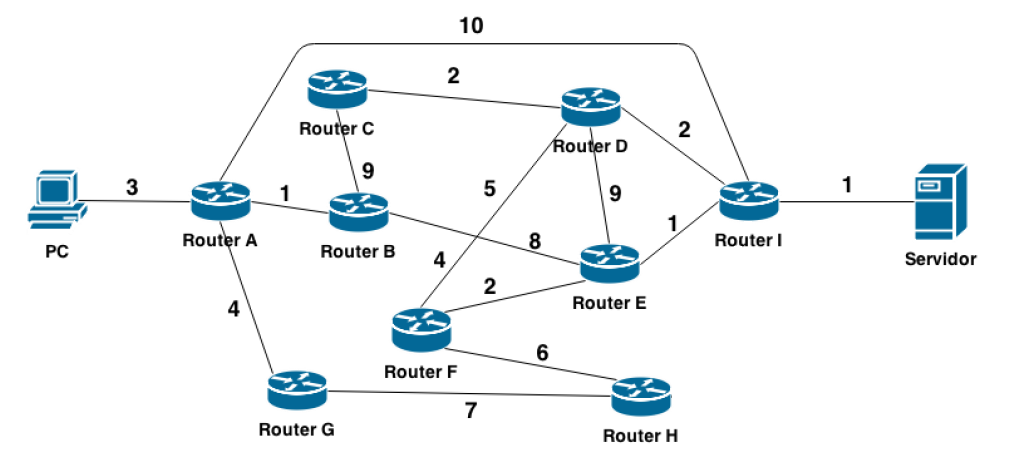
\includegraphics[width=130mm]{mapaderedes.png}
\caption{Red con enlace roto entre nodos H e I.}
\label{overflow}
\end{figure}

\begin{tabular}{||l | c | c | c | c | c | c | c | c | c | c | c ||}
\hline
\hline
O/D & PC & A & B & C & D & E & F & G & H & I & SERVER \\
\hline
PC & 0 & 3 & 4 & 13 & 15 & 12 & 14 & 7 & 14 & 13 & 14 \\
\hline
A & 3 & 0 & 1 & 10 & 12 & 9 & 11 & 4 & 11 & 10 & 11 \\
\hline
B & 4 & 1 & 0 & 9 & 11 & 8 & 10 & 5 & 12 & 9 & 10 \\
\hline
C & 13 & 10 & 9 & 0 & 2 & 5 & 6 & 14 & 7 & 4 & 5 \\
\hline
D & 15 & 12 & 11 & 2 & 0 & 3 & 4 & 12 & 5 & 2 & 3 \\
\hline
E & 12 & 9 & 8 & 5 & 3 & 0 & 2 & 11 & 4 & 1 & 2 \\
\hline
F & 14 & 11 & 10 & 6 & 4 & 2 & 0 & 13 & 6 & 3 & 4 \\
\hline
G & 7 & 4 & 5 & 14 & 12 & 11 & 13 & 0 & 7 & 10 & 11 \\
\hline
H & 14 & 11 & 12 & 7 & 5 & 4 & 6 & 7 & 0 & $\infty$ & 4 \\
\hline
I & 13 & 10 & 9 & 4 & 2 & 1 & 3 & 10 & $\infty$ & 0 & 1 \\
\hline
SERVER & 14 & 11 & 10 & 5 & 3 & 2 & 4 & 11 & 4 & 1 & 0 \\
\hline
\end{tabular}\\\\

Cuando el barco transatl\'antico corta el enlace entre los nodos H e I, el alogoritmo vector distancia se comporta de la siguiente manera:

H marca la distancia a I como $\infty$ y le dice a G,F,E.

Mientras que I marca la distancia a H como $\infty$ y le dice a D, E, SERVER.

$D_h$(PC)=14\\
$D_h$(A)=11\\
$D_h$(B)=12\\
$D_h$(C)=12\\
$D_h$(D)=10\\
$D_h$(E)=8\\
$D_h$(F)=6\\
$D_h$(G)=7\\
$D_h$(I)=9\\
$D_h$(SERVER)=10\\

$D_i$(PC)=13\\
$D_i$(A)=10\\
$D_i$(B)=9\\
$D_i$(C)=4\\
$D_i$(D)=2\\
$D_i$(E)=1\\
$D_i$(F)=3\\
$D_i$(G)=14\\
$D_i$(H)=9\\
$D_i$(SERVER)=1\\

$D_g$(PC)=7\\
$D_g$(A)=4\\
$D_g$(B)=5\\
$D_g$(C)=14\\
$D_g$(D)=min\{16,16\}=16\\
$D_g$(E)=min\{15,13\}=13\\
$D_g$(F)=13\\
$D_g$(H)=7\\
$D_g$(I)=min\{16,14\}=14\\
$D_g$(SERVER)=15\\

$D_f$(PC)=14\\
$D_f$(A)=11\\
$D_f$(B)=10\\
$D_f$(C)=6\\
$D_f$(D)=4\\
$D_f$(E)=2\\
$D_f$(G)=13\\
$D_f$(H)=6\\
$D_f$(I)=3\\
$D_f$(SERVER)=4\\

$D_e$(PC)=12\\
$D_e$(A)=9\\
$D_e$(B)=8\\
$D_e$(C)=5\\
$D_e$(D)=3\\
$D_e$(F)=2\\
$D_e$(G)=min\{15,13\}=13\\
$D_e$(H)=8\\
$D_e$(I)=1\\
$D_e$(SERVER)=2\\

$D_d$(PC)=15\\
$D_d$(A)=12\\
$D_d$(B)=11\\
$D_d$(C)=2\\
$D_d$(E)=3\\
$D_d$(F)=4\\
$D_d$(G)=min\{17,16\}=16\\
$D_d$(H)=min\{10,11\}=10\\
$D_d$(I)=2\\
$D_d$(SERVER)=3\\

$D_s$(PC)=14\\
$D_s$(A)=11\\
$D_s$(B)=10\\
$D_s$(C)=5\\
$D_s$(D)=3\\
$D_s$(E)=2\\
$D_s$(F)=4\\
$D_s$(G)=15\\
$D_s$(H)=10\\
$D_s$(I)=1\\

$D_c$(PC)=13\\
$D_c$(A)=10\\
$D_c$(B)=9\\
$D_c$(C)=2\\
$D_c$(D)=5\\
$D_c$(E)=6\\
$D_c$(F)=14\\
$D_c$(G)=12\\
$D_c$(H)=4\\
$D_c$(I)=5\\

$D_b$(PC)=4\\
$D_b$(A)=1\\
$D_b$(C)=9\\
$D_b$(D)=11\\
$D_b$(E)=8\\
$D_b$(F)=10\\
$D_b$(G)=5\\
$D_b$(H)=12\\
$D_b$(I)=9\
$D_b$(SERVER)=10\\

$D_a$(PC)=3\\
$D_a$(B)=1\\
$D_a$(C)=10\\
$D_a$(D)=12\\
$D_a$(E)=9\\
$D_a$(F)=11\\
$D_a$(G)=4\\
$D_a$(H)=11\\
$D_a$(I)=10\\
$D_a$(SERVER)=11\\

$D_{pc}$(A)=3\\
$D_{pc}$(B)=4\\
$D_{pc}$(C)=13\\
$D_{pc}$(D)=15\\
$D_{pc}$(E)=12\\
$D_{pc}$(F)=14\\
$D_{pc}$(G)=7\\
$D_{pc}$(H)=14\\
$D_{pc}$(I)=13\\
$D_{pc}$(SERVER)=14\\

Tabla actualizada luego de eliminar la conexi\'on entre H e I

\begin{tabular}{||l | c | c | c | c | c | c | c | c | c | c | c ||}
\hline
\hline
O/D & PC & A & B & C & D & E & F & G & H & I & SERVER \\
\hline
PC & 0 & 3 & 4 & 13 & 15 & 12 & 14 & 7 & 14 & 13 & 14 \\
\hline
A & 3 & 0 & 1 & 10 & 12 & 9 & 11 & 4 & 11 & 10 & 11 \\
\hline
B & 4 & 1 & 0 & 9 & 11 & 8 & 10 & 5 & 12 & 9 & 10 \\
\hline
C & 13 & 10 & 9 & 0 & 2 & 5 & 6 & 14 & 12 & 4 & 5 \\
\hline
D & 15 & 12 & 11 & 2 & 0 & 3 & 4 & 16 & 10 & 2 & 3 \\
\hline
E & 12 & 9 & 8 & 5 & 3 & 0 & 2 & 13 & 8 & 1 & 2 \\
\hline
F & 14 & 11 & 10 & 6 & 4 & 2 & 0 & 13 & 6 & 3 & 4 \\
\hline
G & 7 & 4 & 5 & 14 & 16 & 13 & 13 & 0 & 7 & 14 & 15 \\
\hline
H & 14 & 11 & 12 & 12 & 10 & 8 & 6 & 7 & 0 & 9 & 10 \\
\hline
I & 13 & 10 & 9 & 4 & 2 & 1 & 3 & 14 & 9 & 0 & 1 \\
\hline
SERVER & 14 & 11 & 10 & 5 & 3 & 2 & 4 & 15 & 10 & 1 & 0 \\
\hline
\end{tabular}\\\\

En esta secci\'on como se observa solo cambiaron los valores correspondientes a los vecinos de H e I, exceptuando H a I, ya que para el c\'alculo del Vector-Distancia era necesario la conexi\'on entre H e I.
\end{document}
